\documentclass{beamer}
\title{A Perturbative Approach to the Ground State of Interacting Fermions in the Mean Field
Limit}
\author{Filippo Cozzi}


% packages
\usepackage[a-1b]{pdfx}
\usepackage{tikz}
\usetikzlibrary{decorations.markings}
\usetikzlibrary{arrows.meta}


% set up the presentation
\usetheme{Antibes}
\usefonttheme[onlymath]{serif}

\begin{document}
\frame{\titlepage}

\AtBeginSection[]{
	\begin{frame}
		\frametitle{Contents}
		\tableofcontents[currentsection]
	\end{frame}
}


% sections:

\section{The Fermi Gas}

\begin{frame}
	We begin by introducing the system in exam: a Fermi gas with a two-body interaction,
	composed of $N$ particles
	\begin{align*}
		H_N = H_0 + \lambda \sum_{1\leq i<j\leq N} V(x_i-x_j)
	\end{align*}
	where
	\begin{itemize}
		\item $H_0$ is the kinetic energy;
		\item $V$ is the two-body interaction potential:
			\begin{itemize}
				\item[(i)] $V$ is a Schwartz function;
				\item[(ii)] $V$ depends only on $\vert x_i-x_j\vert$;
				\item[(iii)] $\hat{V}$ has compact support;
			\end{itemize}
		\item $\lambda$ is the coupling constant.
	\end{itemize}
\end{frame}

\subsection{The free Fermi gas}

\begin{frame}
	Let us recall the properties of the \textbf{free Fermi gas}. On the fermionic $N$-particle
	state space
	\begin{align*}
		\mathcal{H}_N = \big\{
			&\psi\in L^2(\mathbb{T}^{3N}) : \\
			&\psi(x_1,\ldots,x_N) = (-)^\sigma\psi(x_{\sigma(1)},\ldots,x_{\sigma(N)})
		\big\}
	\end{align*}
	the kinetic energy is the sum of kinetic energies, with a Slater determinant ground state
	\begin{align*}
		H_0 = \sum_{i=1}^N -\hbar^2\Delta_i
		\qquad \Psi_{\mathrm{gs}} = \bigwedge_{k\in B_{\mathrm{F}}}\psi_k
	\end{align*}
	where $\psi_k(x) = (2\pi)^{-3/2}e^{-ik\cdot x}$.
	\begin{block}{Remark}
		$\hbar$ is chosen to be a physical parameter that we will tweak in the mean field
		limit. It is not the foundamental Planck's constant.
	\end{block}
\end{frame}

\begin{frame}
	The Slater determinant is a consequence of Pauli's exclusion principle, manifest in the
	complete antisymmetry of the wave function $\Psi_{\mathrm{gs}}$.

	Momentum states $\psi_k$ can be occupied by at most one particle. The energy
	spectrum is $\epsilon_k = \hbar^2 \vert k\vert^2$: adding particles in the lowest energy
	states available fills a ball in momentum space. \textcolor{red}{FERMI BALL IMAGE}

	The \textbf{Fermi momentum} is the radius of the highest occupied shell
	\begin{align*}
		&k_{\mathrm{F}} = \left(\frac{3}{4\pi}N\right)^{\frac{1}{3}} + \mathcal{O}(1)\\
		&B_{\mathrm{F}} = \left\{ k\in\mathbb{Z}^3 : \vert k\vert\leq k_{\mathrm{F}} \right\}
	\end{align*}
\end{frame}

\subsection{Adding interactions}

\begin{frame}
	Adding interactions introduces non-trivial correlations between particle states, and these
	properties are better understood from a statistical mechanics perspective: at
	thermal equilibrium the ground state energy is the zero temperature limit of the free
	energy.

	\begin{block}{Definition}
		A \textbf{thermal equilibrium state} at inverse temperature $\beta$ is a quantum state
		$\langle\,\cdot\,\rangle_\beta\in\mathcal{B}(\mathcal{H}_N)^*$ that follows the
		Boltzmann distribution $p(\epsilon)=Z^{-1}e^{-\beta\epsilon}$:
		\begin{align*}
			\langle\,\cdot\,\rangle_\beta = \frac{\mathrm{Tr}(\,\cdot\,e^{-\beta H_N})}{Z},
			\qquad Z = \mathrm{Tr}(e^{-\beta H_N}).
		\end{align*}
		$\langle\,\cdot\,\rangle_\beta$ is also called a
		\textit{Gibbs state}.
	\end{block}
\end{frame}

\begin{frame}
	The quantity $Z$ is the \textbf{partition function} and it contains all the information we
	are looking for. The free energy is just
	\begin{align*}
		F = -\frac{\log(Z)}{\beta},\qquad
		E_{\mathrm{gs}} = \lim_{\beta\to\infty} F
	\end{align*}
	so we need to compute $\log(Z)$ first. To carry out such computation we work in the
	\textbf{grand canonical picture}, using the second quantization formalism. When working
	in the grand canonical picture, the energy acquires the additional term $-\mu\mathcal{N}$,
	with $\mu$ being the \textbf{chemical potential}, and $\mathcal{N}$ the number operator.
\end{frame}

\begin{frame}
	In second quantization, $N$ is allowed to vary by modifying the state space to the
	\textbf{Fock space}. For fermions with one-particle state space $\mathfrak{h}$:
	\begin{align*}
		\mathcal{F}^{\mathrm{F}}(\mathfrak{h}) = \bigoplus_{N=0}^\infty \bigwedge_{j=1}^N \mathfrak{h}
	\end{align*}
	with the $N=0$ sector being, conventionally, $\mathbb{C}$.
\end{frame}

\begin{frame}
	On a Fock space, observables are written in terms of \textbf{creation/annihilation}
	operators
	\begin{align*}
		a(f) \varphi_1\otimes\cdots\otimes\varphi_N
		&= \langle f,\varphi_1\rangle \varphi_2\otimes\cdots\otimes\varphi_N\\
		a^*(f)\varphi_1\otimes\cdots\otimes\varphi_N
		&= f\otimes\varphi_1\otimes\cdots\otimes\varphi_N.
	\end{align*}
	Their fermionic version is given by projecting onto the antisymmetric subspace of each
	$N$-particle sector:
	\begin{align*}
		a_-(f) = \sqrt{N}a(f)\qquad a^*_-(f) = \sqrt{N}P_-a^*(f).
	\end{align*}
	\begin{block}{CAR}
		These satisfy the \textbf{Canonical Anticommutation Relations}:
		\begin{align*}
			\{a_-(f),a^*_-(g)\} = \langle f,g\rangle\mathrm{I}
		\end{align*}
		with all other anticommutators being zero.
	\end{block}
\end{frame}

\begin{frame}
	With creation/annihilation operators, the Hamiltonian $H_N$ is lifted to
	$\mathcal{F}^{\mathrm{F}}(\mathfrak{h})$:
	\begin{align*}
		H = \bigoplus_{N=0}^\infty H_N
	\end{align*}
	where
	\begin{align*}
		H_N = \sum_{k\in\mathbb{Z}^3} (\hbar^2\vert k\vert^2 - \mu)a^*_k a_k
		+ \lambda \sum_{p,q,k\in\mathbb{Z}^3} \hat{V}(k)a^*_{p-k}a^*_{q+k} a_q a_p.
	\end{align*}
\end{frame}

\section{Mean Field Limit}

\begin{frame}
	In the free Fermi gas, the Fermi momentum grows as $k_{\mathrm{F}}=\mathcal{O}(N^{-1/3})$.
	Then the total energy in the ground state grows as
	$E^{(0)}_{\mathrm{gs}}=\mathcal{O}(N^{5/3})$.

	Adding the interaction means the potential energy will be of order $N^2$ as the number
	of pair-wise interactions is $N(N-1)/2$.

	\begin{block}{Mean field scaling}
		To get a non-trivial limit for the true ground state energy as $N\to\infty$, we define
		\begin{align*}
			\hbar = N^{-1/3} \quad\textrm{and}\quad \lambda = N^{-1}.
		\end{align*}
	\end{block}
\end{frame}

\begin{frame}
	In this mean field scaling limit, exact methods show that the ground state energy can be
	approximated by
	\begin{align*}
		E_{\mathrm{gs}} = E^{\mathrm{HF}}_N + E^{\mathrm{RPA}}_N
		+ \mathcal{O}(N^{-\frac{1}{3} -\alpha}).
	\end{align*}
	Here
	\begin{itemize}
		\item $E^{\mathrm{HF}}=\mathcal{O}(N)+\mathcal{O}(1)$ is the contribution from the
			\textbf{Hartree-Fock (HF)} approximation;
		\item $E^{\mathrm{RPA}}=\mathcal{O}(N^{-1/3})$ is the contribution from the
			\textbf{Random Phase Approximation (RPA)};
		\item $\alpha>0$ indicates that further contributions will be subleading with respect
			to the RPA.
	\end{itemize}
\end{frame}

\begin{frame}
	Our work introduces rigorous perturbation theory into the picture. We start by the first
	order, and then lay the groundwork for the second.

	\begin{itemize}
		\item The first order approximation leads to the HF term, containing the unperturbed
			energy, the \textbf{direct} ($\mathcal{O}(N)$) and the \textbf{exchange}
			($\mathcal{O}(1)$) corrections;
		\item The RPA contains higher order direct contributions (all expected to be of order
			$\mathcal{O}(N^{-1/3})$);
		\item Already at second order, the exchange contribution is expected to be subleading
			with respect to the RPA, and thus fall in the error term.
	\end{itemize}
\end{frame}

\section{Perturbative Series}

\subsection{Expanding the partition function}

\begin{frame}
	Because $H$ is the sum of a kinetic term and an interaction term, the partition function
	cannot be computed exactly, but we can formally expand it in powers of $\lambda$:
	\begin{block}{Duhamel's formula}
		The following approximation for $\log(Z)$ holds formally at second order in $\lambda$:
		\begin{align*}
			&\log\,\mathrm{Tr}\,e^{-\beta H}=\\
			&= \log\,\mathrm{Tr}\,e^{-\beta H_0} - \lambda\beta\langle V\rangle_\beta\\
			&\quad+ \lambda^2 \int_0^\beta\mathrm{d}\tau\int_0^\tau\mathrm{d}\tau'\,
			\left(\langle V(\tau')V(\tau)\rangle_\beta - \langle V(\tau')\rangle_\beta\langle V(\tau)\rangle_\beta\right)
		\end{align*}
	\end{block}
\end{frame}

\begin{frame}
	In this formula:
	\begin{itemize}
		\item The expectation $\langle\,\cdot\,\rangle_\beta$ is done with respect to the
			kinetic term $H_0$;
		\item $V(\tau) = e^{-\tau H_0}Ve^{\tau H_0}$ is the ``evolution" of $V$ at inverse
			temperature $\tau$;
		\item $Z_0=\log\,\mathrm{Tr}\,e^{-\beta H_0}$ is just the partition function for the
			free system\\
			$\implies$ terms in $\lambda$ and $\lambda^2$ are higher order corrections to $Z_0$.
	\end{itemize}

	The expectations $\langle V\rangle_\beta$ and $\langle V(\tau')V(\tau)\rangle_\beta
	-\langle V(\tau')\rangle_\beta\langle V(\tau)\rangle_\beta$ can be computed using
	\textbf{Wick's theorem}.
\end{frame}

\subsection{Feynman diagrams}

\begin{frame}
	\begin{block}{Wick's theorem}
		If $H = \sum_{k}\epsilon_k a^*_ka_k$ with $\sum_ke^{-\beta\epsilon_k}<\infty$, then,
		given a family of creation and annihilation operators $A_1,\ldots,A_{2n}$, it holds
		that
		\begin{gather*}
			\langle A_1\cdots A_{2n}\rangle_\beta =
			\sum_{\sigma\in P_{2n}}(-1)^\sigma\prod_{j=1}^{2n-1}
			\langle A_{\sigma(j)}A_{\sigma(j+1)}\rangle_\beta\\
			\langle A_1\cdots A_{2n-1}\rangle_\beta = 0
		\end{gather*}
		where $P_{2n}$ is the set of \textbf{pairings} of $2n$ elements.
	\end{block}
	\begin{block}{Remark}
		Wick's theorem is the defining property of \textbf{quasi-free states}. Gibbs states
		for quadratic Hamiltonians are quasi-free.
	\end{block}
\end{frame}

\begin{frame}
	Wick's theorem can be used diagrammatically:
	\begin{itemize}
		\item to a two-point function $\langle a^*_k(\tau)a_{k'}(\tau')\rangle_\beta$ is
			associated the \textbf{propagator $G_{k,k'}(\tau,\tau')$}:
			\begin{align*}
				G_{k,k'}(\tau,\tau') =
				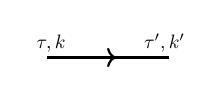
\begin{tikzpicture}[scale=.6, baseline=(current bounding box.south)]
					\node (a) at (-1.5,0) {} node[scale=0.7] at (-1.2,0.3) {$\tau,k$};
					\node (b) at ( 1.5,0) {} node[scale=0.7] at ( 1.2,0.3) {$\tau',k'$};
					\begin{scope}[very thick, decoration={
							markings,
							mark=at position 0.57 with {\arrow{>}}}
						]
						\draw[black, thick, postaction={decorate}] (a) -- (b);
					\end{scope}
				\end{tikzpicture}
			\end{align*}
		\item to the interaction term is associated a \textbf{vertex}:
			\begin{align*}
				\sum_{p,q,k}\hat{V}(k)a^*_{p-k}a^*_{q+k}a_qa_p =
				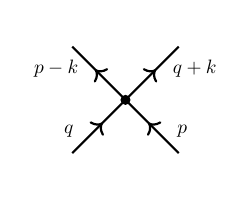
\begin{tikzpicture}[scale=.8, baseline=(current bounding box.center)]
					\node (a) at (-1, 1) {} node[scale=0.7] at (-1.1, 0.5) {$p-k$};
					\node (b) at ( 1, 1) {} node[scale=0.7] at ( 1.1, 0.5) {$q+k$};
					\node (c) at (-1,-1) {} node[scale=0.7] at (-0.9,-0.5) {$q$};
					\node (d) at ( 1,-1) {} node[scale=0.7] at ( 0.9,-0.5) {$p$};
					\begin{scope}[very thick, decoration={
							markings,
							mark=at position 0.57 with {\arrow{>}}}
						]
						\draw[black, thick, postaction={decorate}] (0,0) -- (a);
						\draw[black, thick, postaction={decorate}] (0,0) -- (b);
						\draw[black, thick, postaction={decorate}] (c) -- (0,0);
						\draw[black, thick, postaction={decorate}] (d) -- (0,0);
					\end{scope}
					\filldraw[black] (0,0) circle (2pt);
				\end{tikzpicture}
			\end{align*}
		\item propagators connect vertices to form a \textbf{Feynman diagram}.
	\end{itemize}
\end{frame}

\begin{frame}
	\begin{block}{Linked cluster theorem}
		For a product of $n$ vertices $V_1,\ldots,V_n$, we have the following identity in
		terms of values of \textbf{connected Feynman diagrams}:
		\begin{align*}
			\langle V_1\cdots V_n\rangle_\beta - \langle V_1\rangle_\beta\cdots\langle V_n\rangle_\beta
			= \sum_{\Gamma\in\mathcal{G}_{n,\mathrm{C}}}\mathrm{val}(\Gamma),
		\end{align*}
		where $\mathcal{G}_{n,\mathrm{C}}$ is the set of all connected Feynman diagrams that
		contain $n$ vertices.
	\end{block}
	Looking at the second order expansion of $\log(Z)$:
	\begin{itemize}
		\item At first order: $\langle V\rangle_\beta$ is the sum of all connected Feynman
			diagrams with \textit{one vertex};
		\item At second order: $\langle V(\tau')V(\tau)\rangle_\beta-
			\langle V(\tau')\rangle_\beta\langle V(\tau)\rangle_\beta$ is the sum of all
			connected Feynman diagrams with \textit{two vertices}.
	\end{itemize}
\end{frame}

\section{Main Result}

\subsection{First order}

\begin{frame}
	First, we explicitly evaluate all Feynman diagrams that appear at first order:
	\begin{align*}
		\langle V\rangle_\beta
		&= 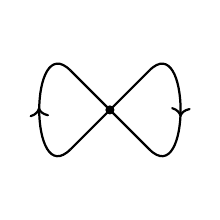
\begin{tikzpicture}[scale=.5, baseline=(current bounding box.center)]
			\node[shape=coordinate] (a) at (-1, 1) {};
			\node[shape=coordinate] (b) at ( 1, 1) {};
			\node[shape=coordinate] (c) at (-1,-1) {};
			\node[shape=coordinate] (d) at ( 1,-1) {};
			\draw[thick] (0,0) -- (a);
			\draw[thick] (0,0) -- (b);
			\draw[thick] (0,0) -- (c);
			\draw[thick] (0,0) -- (d);
			\filldraw[black] (0,0) circle (.1);
			\begin{scope}[very thick, decoration={
					markings,
					mark=at position 0.55 with {\arrow{<}}}
				]
				\draw[thick, postaction={decorate}] (a) .. controls +(135:1.5) and +(225:1.5) .. (c);
			\end{scope}
			\begin{scope}[very thick, decoration={
					markings,
					mark=at position 0.55 with {\arrow{>}}}
				]
				\draw[thick, postaction={decorate}] (b) .. controls +( 45:1.5) and +(315:1.5) .. (d);
			\end{scope}
		\end{tikzpicture}
		+ 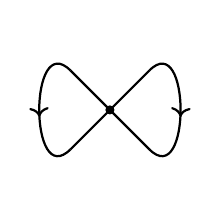
\begin{tikzpicture}[scale=.5, baseline=(current bounding box.center)]
			\node[shape=coordinate] (a) at (-1, 1) {};
			\node[shape=coordinate] (b) at ( 1, 1) {};
			\node[shape=coordinate] (c) at (-1,-1) {};
			\node[shape=coordinate] (d) at ( 1,-1) {};
			\draw[thick] (0,0) -- (a);
			\draw[thick] (0,0) -- (b);
			\draw[thick] (0,0) -- (c);
			\draw[thick] (0,0) -- (d);
			\filldraw[black] (0,0) circle (.1);
			\begin{scope}[very thick, decoration={
					markings,
					mark=at position 0.55 with {\arrow{>}}}
				]
				\draw[thick, postaction={decorate}] (a) .. controls +(135:1.5) and +(225:1.5) .. (c);
				\draw[thick, postaction={decorate}] (b) .. controls +( 45:1.5) and +(315:1.5) .. (d);
			\end{scope}
		\end{tikzpicture}\\
		&= \sum_{p,k\in\mathbb{Z}^3}\left(\hat{V}(0)-\hat{V}(k)\right)n_pn_{p-k}.
	\end{align*}
	Here, the $\hat{V}(0)$ is the order direct term, while $\hat{V}(k)$ is the exchange term.
\end{frame}

\begin{frame}
	\begin{block}{Lemma}
		The series $\sum_{p,k}(\hat{V}(0)-\hat{V}(k))n_pn_{p-k}$ converges uniformly in
		$\beta$ (away from zero).
	\end{block}
	\begin{block}{Theorem: mean field scaling of $E^{\mathrm{HF}}_N$}
		The ground state energy of the interacting Fermi gas in the mean field limit exhibits
		the following scaling in $N$:
		\begin{align*}
			E^{\mathrm{HF}}_N
			&= \lim_{\beta\to\infty}\left(
				-\frac{\log(Z_0) - \lambda\beta\langle V\rangle_\beta}{\beta}
			\right)\\
			&= E^{(0)}_N + \sum_{k\in\mathbb{Z}^3}\sum_{\substack{p\in B_{\mathrm{F}}:\\p-k\in B_{\mathrm{F}}}}\left(\hat{V}(0) - \hat{V}(k)\right)\\
			&= \mathcal{O}(N) + \mathcal{O}(1).
		\end{align*}
	\end{block}
\end{frame}

\subsection{A first attempt at second order}

\begin{frame}
	At second order, the connected Feynman diagrams are split into two possible topologies:
	\begin{figure}[h]
		\begin{minipage}[t]{.48\textwidth}
			\centering
			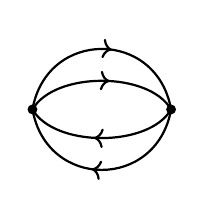
\begin{tikzpicture}[scale=.8, baseline=(current bounding box.center)]
				\node[shape=coordinate] (a) at (-1.1,0) {};
				\node[shape=coordinate] (b) at ( 1.1,0) {};
				\begin{scope}[very thick, decoration={
						markings,
						mark=at position 0.55 with {\arrow{>}}}
					]
					\filldraw[] (-1.1,0) circle (.05);
					\filldraw[] ( 1.1,0) circle (.05);
					\draw[thick, postaction={decorate}] (a) .. controls +( 80:1.3) and +(100:1.3) .. (b);
					\draw[thick, postaction={decorate}] (b) .. controls +(260:1.3) and +(280:1.3) .. (a);
					\draw[thick, postaction={decorate}] (a) .. controls +( 60:0.7) and +(120:0.7) .. (b);
					\draw[thick, postaction={decorate}] (b) .. controls +(240:0.7) and +(300:0.7) .. (a);
				\end{scope}
			\end{tikzpicture}

			\vspace{0.8em}
			\textbf{No tadpoles}
		\end{minipage}
		\hfill
		\begin{minipage}[t]{.48\textwidth}
			\centering
			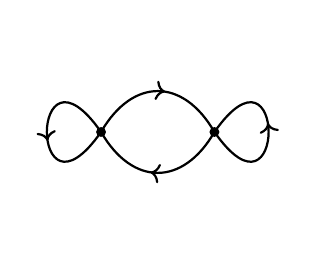
\begin{tikzpicture}[scale=.8, baseline=(current bounding box.center)]
				\node[shape=coordinate] (a) at (-0.9,0) {};
				\node[shape=coordinate] (b) at ( 0.9,0) {};
				\begin{scope}[very thick, decoration={
						markings,
						mark=at position 0.55 with {\arrow{>}}}
					]
					\filldraw[] (-0.9,0) circle (.05);
					\filldraw[] ( 0.9,0) circle (.05);
					\draw[thick, postaction={decorate}] (a) .. controls +(125:2) and +(235:2) .. (a);
					\draw[thick, postaction={decorate}] (b) .. controls +(305:2) and +( 55:2) .. (b);
					\draw[thick, postaction={decorate}] (a) .. controls +( 60:1) and +(120:1) .. (b);
					\draw[thick, postaction={decorate}] (b) .. controls +(240:1) and +(300:1) .. (a);
				\end{scope}
			\end{tikzpicture}

			\textbf{Two tadpoles}
		\end{minipage}
	\end{figure}
	We expect the first kind of diagrams to represent the direct and the exchange
	contributions, while the tadpole diagrams to contribute exactly zero.
\end{frame}

\begin{frame}
	However, we set our calculations in formal perturbation theory. In the fermionic
	case this involves using \textbf{Grassmann variables} and \textbf{Grassmann integrals} to
	reproduce Wick's theorem.

	In $\langle V(\tau)V(\tau')\rangle_\beta$ the vertices are at different
	temperatures: in formal perturbation theory, one should introduce $\tau$-ordering to
	reproduce Duhamel's formula.

	\begin{block}{Remark}
		It may be that the correct perturbations at orders $\geq2$ cannot be obtained without
		looking deeper into the identification between the operatorial and Grassmannian
		perturbative series.
	\end{block}
\end{frame}

\begin{frame}
	Indeed, if we evaluate tadpole diagrams we obtain \textbf{divergent contributions} after
	applying Duhamel's formula.
	\begin{block}{Example: tadpole divergence}
		\begin{align*}
			\lim_{\beta\to\infty}\frac{\beta}{2}\left(
			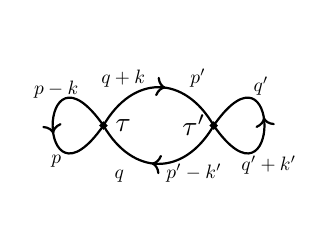
\begin{tikzpicture}[scale=.5, baseline=(current bounding box.center)]
				\node[shape=coordinate] (a) at (-1.4,0) {} node[scale=1] at (-0.9,0) {$\tau$};
				\node[shape=coordinate] (b) at ( 1.4,0) {} node[scale=1] at ( 0.9,0) {$\tau'$};
				\node[scale=0.7] (m1) at (-2.6, 0.9) {$p-k$};
				\node[scale=0.7] (m2) at (-0.9, 1.2) {$q+k$};
				\node[scale=0.7] (m3) at (-2.6,-0.9) {$p$};
				\node[scale=0.7] (m4) at (-1.0,-1.3) {$q$};
				\node[scale=0.7] (n1) at ( 2.6, 1.0) {$q'$};
				\node[scale=0.7] (n2) at ( 1.0, 1.2) {$p'$};
				\node[scale=0.7] (n3) at ( 2.8,-1.0) {$q'+k'$};
				\node[scale=0.7] (n4) at ( 0.9,-1.2) {$p'-k'$};
				\begin{scope}[very thick, decoration={
						markings,
						mark=at position 0.55 with {\arrow{>}}}
					]
					\filldraw[] (a) circle (.05);
					\filldraw[] (b) circle (.05);
					\draw[thick, postaction={decorate}] (a) .. controls +(125:3) and +(235:3) .. (a);
					\draw[thick, postaction={decorate}] (b) .. controls +(305:3) and +( 55:3) .. (b);
					\draw[thick, postaction={decorate}] (a) .. controls +( 60:1.5) and +(120:1.5) .. (b);
					\draw[thick, postaction={decorate}] (b) .. controls +(240:1.5) and +(300:1.5) .. (a);
				\end{scope}
			\end{tikzpicture}\right)
			&= \lim_{\beta\to\infty}\left( -\frac{\beta}{2}\sum_{p,q,k}\hat{V}(0)n_q^2n_pn_{k} \right)\\
			&= -\infty
		\end{align*}
	\end{block}
\end{frame}

\begin{frame}
	Furthermore, diagrams that contribute to the RPA term break the expected scaling in $N$.
	\begin{block}{Example: second order direct contribution}
		\begin{align*}
			E_{\mathrm{D}}^{(2)}
			&= -2\lambda^2 \sum_{k\in\mathbb{Z}^3} \sum_{\substack{p,q\in B_{\mathrm{F}}:\\q+k,p-k\in B_{\mathrm{F}}}}
			\frac{\hat{V}(k)^2}{\hbar^2((p-k)^2+(q+k)^2-q^2-p^2)}\\
			&= \mathcal{O}(N^{1/3}).
		\end{align*}
	\end{block}
\end{frame}

\end{document}
